\documentclass[acmtog, authorversion]{acmart} % twocolumn
\usepackage{graphicx}
\usepackage{subcaption}
\usepackage{todonotes}
\usepackage{hyperref}
\usepackage{etoolbox}
\usepackage{fancyhdr}
\usepackage{float}

\AtBeginDocument{%
  \providecommand\BibTeX{{%
    \normalfont B\kern-0.5em{\scshape i\kern-0.25em b}\kern-0.8em\TeX}}}

\setcopyright{acmlicensed}
\copyrightyear{2018}
\acmYear{2018}

\begin{document}

\title{Trainieren Neuronaler Netze zur Klimavorhersage}

\author{Torge Schwark}
\email{stu236894@mail.uni-kiel.de}
\orcid{1234-5678-9012}
\author{Joschua Quotschalla}
\authornotemark[1]
\email{stu235352@mail.uni-kiel.de}


\maketitle

\section{Einleitung}
Der Klimawandel stellt zweifellos eine der größten Herausforderungen des 21. Jahrhunderts dar. Der rapide Anstieg globaler Durchschnittstemperaturen und die daraus resultierenden Auswirkungen auf Umwelt und Gesellschaft erfordern dringendes Handeln. Als Grundlage für präventive Maßnahmen ist ein umfassendes Verständniss und das erkennen langfristiger Klimatrends zwingend notwendig. 
Die Anwendung neuronaler Netze verspricht nicht nur verbesserte Vorhersagegenauigkeit, sondern eröffnet auch die Möglichkeit, bisher unbekannte Muster und Trends zu identifizieren, die für ein umfassenderes Verständnis des Klimawandels von entscheidender Bedeutung sind.

\subsection{Schwerpunkt: Das Training Neuronaler Netze}
Der Fokus dieser Untersuchung liegt auf dem Training neuronaler Netze, um eine möglichst hohe Vorhersagegenauigkeit zu erzielen. Dabei werden die Architekturtypen MLP, ConvNet, LSTM und Transformer darauf trainiert, eine Klimavorhersage über 25 Jahre zu treffen. Anschließend werden die Ergebnisse analysiert und die Performance der trainierten neuronalen Netze miteinander verglichen. 

\subsection{Ziel}
Das Ziel besteht darin, mithilfe des besten neuronalen Netzes eine aussagekräftige Vorhersage für die Klimaentwicklung der nächsten 100 Jahre zu treffen.
Die folgenden Abschnitte werden detailliert auf die verwendeten Methoden, die Datenaufbereitung, den Trainingsprozess, die Ergebnisse, Anwendung und die abschließende Schlussfolgerung eingehen.

\section{Methoden}

\subsection*{Datensatz und Datenaufbereitung}
\begin{itemize}
    \item Umfassende Analyse des Datensatzes: Histogramme, Barcharts, Landkarten.
    \item Überprüfung auf Duplikate, insbesondere gleiche Städte.
    \item Aufteilung in Trainings- und Validierungssets (70/30).
    \item Filterung von Zeiträumen mit konstanten Daten über 95 Jahre.
\end{itemize}

\subsection*{Training der neuronalen Netze}
\begin{itemize}
    \item Berechnung des MAE über 720 menschliche Vorhersagen als Bezugsgröße.
    \item Anwendung einer Grid Search-Methode für MLPs, ConvNets, LSTMs.
    \item Fine Tuning: Anpassung von Hyperparametern, Augmentation, Normalisierung.
\end{itemize}

\subsection*{Auswertung}
\begin{itemize}
    \item Prüfen auf Overfitting, Analyse des Loss Graphen.
    \item Vergleich des MAE mit menschlichen Vorhersagen.
    \item Analyse der Genauigkeit an Beispielen.
\end{itemize}

\subsection*{Anwendung}
\begin{itemize}
    \item Anwendung des besten Netzwerks für Vorhersagen bis 2110.
    \item Erstellung eines Durchschnittsgraphen von 1750 bis 2110 mittels rolling prediction.
\end{itemize}

\section{Datensatz}
\subsection{Einführung und Datenverständnis}
Die Grundlage dieser Studie bildet der \href{https://www.kaggle.com/datasets/berkeleyearth/climate-change-earth-surface-temperature-data?select=GlobalLandTemperaturesByCity.csv}{"Climate Change: Earth Surface Temperature"} Datensatz.
Der genannte Datensatz umfasst insgesamt 10.064.718 monatliche Durchschnittstemperaturen, die in 3.448 Städten von 159 Ländern erhoben wurden (vgl. Fig. 1)
\begin{figure}[htp]
    \flushleft
    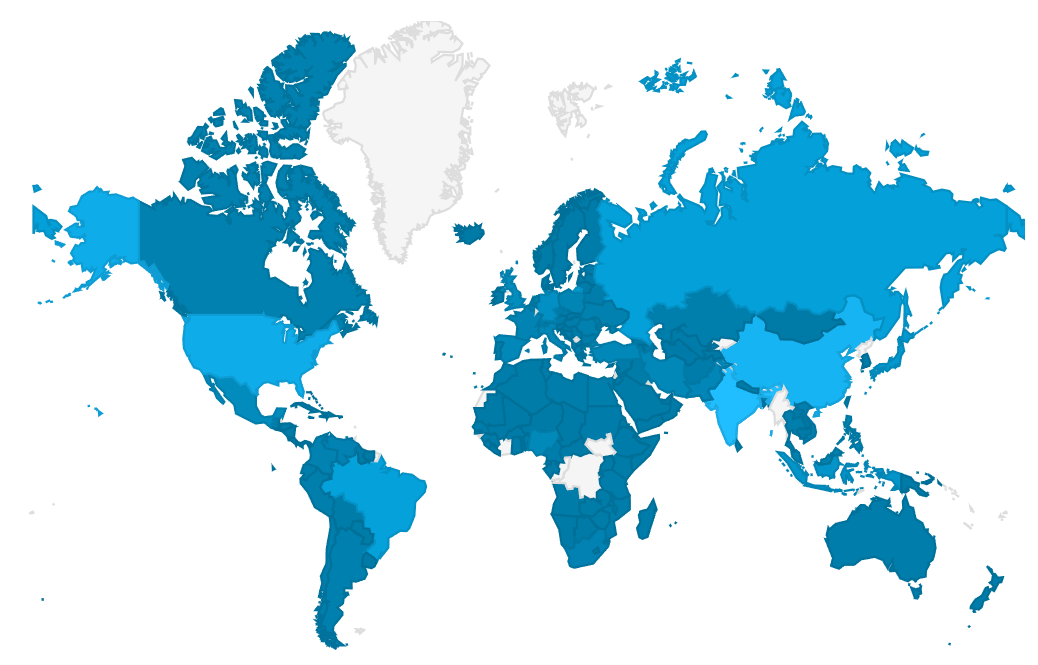
\includegraphics[width=\linewidth]{./map}
    \caption{Ursprung Daten (helleres Blau entspricht mehr Daten)}
    \label{fig:sub1}
\end{figure}

Die Aufzeichnungen reichen dabei von den frühesten Daten im Jahr 1743 bis zu den aktuellsten im Jahr 2015.

\subsection{Fehlende Daten und Ungenauigkeiten}
Bei der Analyse auf Duplikate wurde festgestellt, dass 117 Städte im Datensatz doppelt oder mehrfach vorkommen. Duplikate wurden erkannt, wenn die Daten zweier Städte vollständig identisch sind. Diese doppelten Einträge sind vermutlich darauf zurückzuführen, dass der Datensatz eine Zusammenstellung von 16 bereits bestehenden Datenarchiven darstellt. Zusätzlich zu den durchschnittlichen Temperaturen sind im Datensatz auch die durchschnittlichen Messunsicherheiten für jede Region aufgeführt. Obwohl diese Unsicherheiten stetig abnehmen, stellen sie dennoch eine Herausforderung für die Vorhersagegenauigkeit dar (vgl. Fig. 2).
\begin{figure}[htp]
    \flushleft
    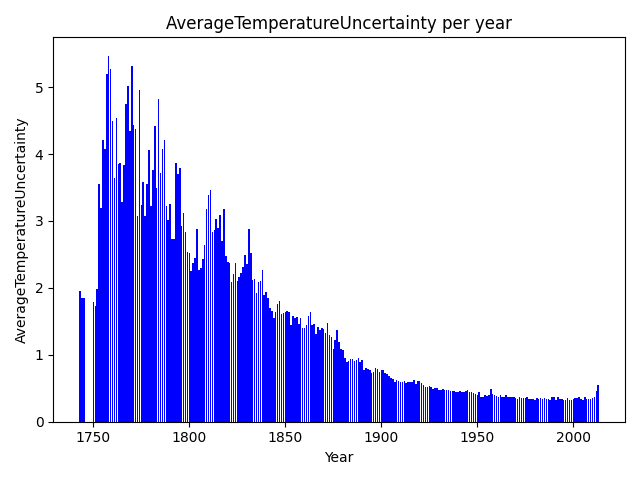
\includegraphics[width=\linewidth]{./Uncertainty_per_year}
    \label{fig:sub2}
    \caption{Messunsicherheit pro Jahr}
\end{figure}
Dabei ist zu berücksichtigen, dass der exakte Messwert mit hoher Wahrscheinlichkeit eine geringere Abweichung aufweist als die Messunsicherheit. Daher ist der durchschnittliche Messfehler deutlich kleiner als die Messunsicherheit. Dies bedeutet, dass der Zufallsfaktor, der durch ungenaue Messungen entsteht und eine untere Grenze für die Vorhersagegenauigkeit bildet, nicht der angegebenen Messunsicherheit entspricht.


\subsection{Data-Loader Pipeline} % noch überarbeiten
Die Data-Loader-Pipeline wurde implementiert, um Mini-Batches von Sequenzen von Datenpunkten gemäß den Anforderungen der Architekturen bereitzustellen. Dabei wird sichergestellt, dass Datenpunkte für die gesamte Inputlänge von 70 Jahren (840 Monaten) und Outputlänge von 25 Jahren (320 Monaten) ohne Lücken vorhanden sind (vgl. Fig. 3).
\begin{figure}[htp]
    \flushleft
    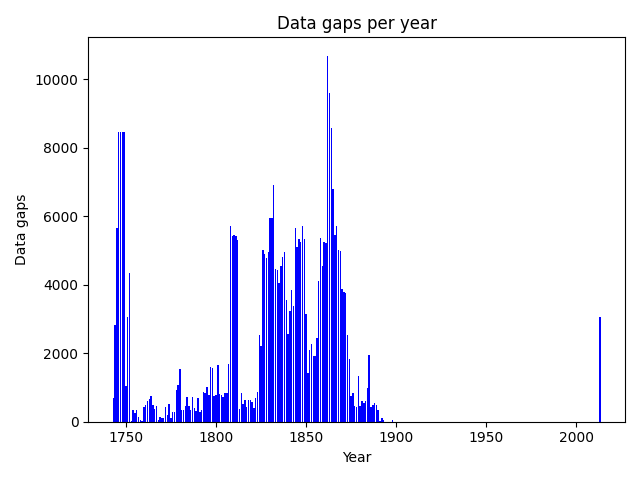
\includegraphics[width=\linewidth]{./Data_gaps}
    \label{fig:sub3}
    \caption{Messunsicherheit pro Jahr}
\end{figure}
Um die Trainings-Effizienz zu steigern, erfolgte die Extraktion der Daten aus den fünf CSV-Dateien, wobei für jeden Standort eine eigene Textdatei erstellt wurde. Zu Beginn wurde ein zufälliger Standort ausgewählt, sowie ein Zeitraum mit vollständigen Messwerten über 90 Jahre.

In einem weiteren Schritt wurde versucht, den Data-Loader weiter zu optimieren, indem die gesamten Daten zunächst in Listen gespeichert und die Suche nach passenden Zeiträumen einmalig zu Beginn des Trainings durchgeführt wurde. Leider brachte diese Optimierung keine Verbesserung.

Die spätere Implementierung von Multiprocessing zur Ausführung des Data-Loaders mit bis zu 20 Prozessen gleichzeitig beschleunigte den Data-Loader mit minimalem Aufwand um etwa das Zehnfache und führte zu einer spürbaren Erhöhung der Hardware-Auslastung.
\section{Training-Procedure} 

Um Klimaprognosen zu erstellen wurden die Architekturtypen MLP, ConvNet, LSTM und Transformer trainiert, auf einem Input von 70 Jahren(840 Monaten) eine Vorhersage für die Nächsten 25 Jahre(300 Monate) zu treffen. Dazu wurden Daten verwendet die Weit genug zurück liegen um die Prognosen mit bereits aufgenommenen Messwerten abgleichen zu können.
Im ersten Schritt wurde eine Grid Search durchgeführt, um optimale Modelle und deren Hyperparameter für die jeweiligen Architekturtypen zu approximieren. Nach dieser automatisierten Suche erfolgte ein manuelles Fine-Tuning, um die Leistung der Modelle weiter zu verbessern. 

\subsection{Optimierung von Architekturen und Parametern}
Im Rahmen der Untersuchung wurden verschiedene Hyperparameter betrachtet und optimiert, um bestmögliche Ergebnisse zu erzielen. Hierzu zählten allgemeine Parameter wie die Batchsize, die Anzahl der Epochen, die Steps pro Epoche, die Anzahl der Validierungssteps und das Verhältnis von Trainingsdaten zu Validierungsdaten. Darüber hinaus besitzen die genannten Architekturen eigene Charakteristiken, die einen erheblichen Einfluss auf die Performance haben. Diese werden im folgenden genauer untersucht.

\subsection{Allgemeine Parameter / Settings}

Da im Training als erstes eine Grid Search durchgeführt wurde und in dieser ausschließlich die Auswirkung der verschiedener Architekturen, Batch sizes und Learning rates auf den MAE untersucht wurden, mussten die restlichen Parameter zunächst festgelegt werden. Dabei wurde sich auf die bereits erwähnte Input- und Output-Länge, die Aufteilung des Datensatzes in 70 Prozent zum Trainieren und 30 Prozent zum Validieren und die Patience von 10 Epochen geeinigt. Durch die Patience wird sichergestellt, dass das Training erst nach 10 Epochen ohne eine Verbesserung des MAEs beendet wird. Des Weiteren wurden damit die Geschwindigkeit des Trainings vergleichbar bleibt die Steps/Epoche dynamisch an die Batch size angepasst, sodass unabhängig von der Batch Size, pro Epoche die gleiche Menge an Daten betrachtet werden. In der späteren Auswertung wird jedoch deutlich, dass selbst dieser Ansatz zur Vergleichbarkeit der Ergebnisse bei unterschiedlichen Batch-Größen nicht zwingend gerecht ist. Außerdem wurden Augmentation und Normalisierung in der Grid Search bisher noch nicht berücksichtigt.

\subsection{Vergleichsmetrik}
Als Vergleichswert für die Vorhersagegenauigkeit dient im Folgenden der MAE. Dieser wurde anstelle des MSE gewählt, da die Zufälligkeit von Temperaturdaten dazu führt, dass eine quadratische Berechnung des Fehlers weniger sinnvoll ist als ein Durchschnittswert. Der MAE stellt in diesem Kontext einen Wert für die durchschnittliche Abweichung in Grad Celsius dar.

\subsection{Grid Search}
\subsubsection{Training Mlps: }
Im Kontext von Multilayer-Perzeptronen (MLPs) spielen vor allem die Anzahl der Hidden Layer in Kombination mit der Dropout-Rate und die Anzahl der Neuronen pro Layer eine entscheidende Rolle bei der Optimierung. In der Grid Search wurden zunächst die folgenden Architekturen trainiert:
\begin{itemize}
    \item MLP1: 500, 200, 200, 400
    \item MLP2: 500, 500, 500, 500, 500, 500, 500, 500, 500
    \item MLP3: 1500, 1500, 1500, 1500, 1500
\end{itemize}
Das erste neuronale Netz (NN) war ein Multilayer-Perzeptron (MLP) mit insgesamt 4 Layern. Dabei umfasste die erste Schicht 500 Neuronen, die zweite 200 Neuronen und so weiter. Die Learning Rate wurde dabei zwischen 0,001, 0,0005, 0,0001 und 0,000005 variiert. Die Batch-Größen wurden zwischen 25, 50, 100 und 200 gewählt.
\subsubsection{Training ConvNets: }
Für 1D-ConvNets sind insbesondere die Größe und Anordnung der Filter sowie deren Anzahl in den Convolutional Layern und das darauf folgende MLP von großer Bedeutung. 
In der Grid Search wurden zunächst die folgenden Architekturen trainiert:
\begin{itemize}
    \item ConvNet1: Anzahl: 10, 10, 10, Größe: 5,5,5 
    \item ConvNet2: Anzahl: 20, 20, 20, 20, 20, Größe 30, 30, 30, 30, 30
    \item ConvNet3: Anzahl: 50, 50, 50, 50, 50, Größe 10, 20, 20, 20, 10
    \item ConvNet4: Anzahl: 50, 50, 50,  Größe 10, 10, 10
\end{itemize}
Das ConvNet1 hat also 3 layer mit jeweils 10 Filtern der Größe 5.
Die Learning Rate wurde zwischen 0.002, 0.001, 0.0004 und 0.0001 variiert. Die Batch-Größe wurde zwischen 25, 50, 75 und 100 gewählt.
Auf die ConvNet schichten folgten 4 Dense Layer der Form 400, 300, 200, 100 die in der Automatisierten Suche nicht weiter angepasst wurden.
\subsubsection{LSTMs (Long Short-Term Memory Networks) :}
Bei den LSTMs hingegen ist ein zentraler Parameter die Anzahl der Memory Units pro Layer. In der Grid Seach wurden zunächst die folgenden Architekturen trainiert:
\begin{itemize}
    \item LSTM1: 10, 10, 10, 10 Dense: 100,50
    \item LSTM2: 20, 20, 20, 20, 20, 20, 20, 20 Dense: 100, 90, 80, 70, 60, 50
    \item LSTM3: 30, 30, 30, 30, 30 Dense: 200,100
    \item LSTM4: 100, 100, 100, 100, 100 Dense: 500,250
\end{itemize}
So hat das erste LSTM 4 Layer mit jeweils 10 LSTM Units und 2 nachfolgende Dense Layer der Form 500, 250. Die Learning Rate wurde dabei zwischen 0,05, 0.03, 0.01 und 0.005 Variiert. Die Batch Size zwischen 25, 50, 75 und 100.

\subsection{Fine Tuning}
Nach der Grid Search wurde ein zusätzliches Fine Tuning für die drei Architekturen MLP, ConvNet und LSTM durchgeführt. Dabei wurden die Parameter der jeweils besten Neuronalen Netze der Grid Search weiter optimiert, und zusätzlich bisher unberücksichtigte Parameter eingestellt. Für die Data Augmentation schien das Hinzufügen eines Gaus verteilten Zufallsfaktors keinen Sinn zu ergeben, stattdessen wurde eine Gaus-Verteilte Skalierung um einen Faktor zwischen 0.5 und 2 und ebenfalls eine Gausverteilte Transformation um einen Faktor zwischen -10 und 10 vorgenommen. Somit konnten noch stärkere Temperatur Extrema, Stätigere oder noch Variierendere Temperaturen trainiert werden.
Aufgrund des Zeitaufwandes wurde für die Transformer keine Grid Search durchgeführt. Das Finden einer möglichst performanten Architektur wurde hier ausschließlich durch menschliche Einstellungen bestimmt.  


\section{Ergebisse}

\subsection{Grid Search Ergebnisse}

Für alle MLPs sahen die Ergebnisse der Grid Search ähnlich aus. Hier beispielhaft für das MLP3 der MAE bei verschiedener Learning Rate und Batch Size:
\begin{figure}[H]
    \flushleft
    \includegraphics[width=0.9\linewidth]{./MLP3}
    \label{fig:sub4}
    \caption{Grid Search MLP3}
\end{figure}
Der Fehler(MAE) war für alle drei Architekturen und jede gewählte Einstellung sehr niedrig. für die MLPs wurde dabei ein minimaler Fehler von 0.88 mit dem MLP2 das den folgendem Aufbau hatte, erreicht: 
\begin{figure}[H]
    \centering
    \includegraphics[width=0.7\linewidth]{./MLP2}
    \label{fig:sub5}
    \caption{Aufbau MLP2}
\end{figure}
Im Fine Tuning hat sich herausgestellt, das mit einer etwas kleineren Architektur, längerem Training und einer größeren Batch Size als aus der Grid Search hervorgegangen ist eine Performance von MAE = 0.836 erreicht werden konnte. Dabei hat die Augmentation eine weitere Verbesserung erbracht.
Auch für die ConvNets waren die Ergebnisse äußerst Stabil. In dem Folgenden Diagramm ist der MAE beispielhaft für das ConvNet2 über verschiedene Batch Sizes und Learning Rate zu sehen:
\begin{figure}[H]
    \centering
    \includegraphics[width=0.9\linewidth]{./ConvNet2}
    \label{fig:sub6}
    \caption{Grid Search ConvNet2}
\end{figure}
Den niedrigsten MAE erreichte ConvNet1 dieser lag nach der Grid Search bei 0.86. Durch das Fine Tuning konnte die Genauigkeit auf 0.83 verbessert werden. dabei sorgten vor allem eine größere Batch Size eine angepasste Learning Rate, längeres Training als auch Augementation für noch bessere Ergebnisse.
Das Traing für die LSTMs sah jedoch deutlich anders aus. Nicht alle Architekturen performten gut, viele Trainings endeten mit einem MAE von 5 oder höher. Wie in dem beispielhaften Diagramm für Das LSTM4 zu sehen ist brachten nur wenige Konfigurationen Erfolge:
\begin{figure}[H]
    \centering
    \includegraphics[width=0.9\linewidth]{./LSTM4}
    \label{fig:sub7}
    \caption{Grid Search LSTM4}
\end{figure}
Obwohl das beste LSTM(LSTM3) nach der Grid Search insgesamt das Netzwerk mit dem 89. besten MAE war, lag der Fehler bei etwa 1.1 Grad Celsius(MAE) und konnte durch das Fine Tuning wiedererwartend auf bis 0.88 verbessert werden.

\subsubsection{Trainingsdauer}
Auch im Bezug auf die Trainingsdauer und Vorhersagegeschwindigkeit lassen sich Unterschiede zwischen den verschiedenen Architekturen feststellen. 
Dies ist vor allem anhand der Komplexität der Modelle und den benötigten Berechnungen geschuldet, welche mehr oder weniger häufig und parallel ablaufen können.
So brauchten 1D-ConvNets als auch MLPs im Schnitt nur etwa 3 Sekunden pro Epoche die LSTMs und Transformer hingegen etwa 25 Sekunden.
Im Zusammenhang mit bis zu 300 Epochen, über die manche Netzwerke trainiert wurden machen sich somit deutliche Differenzen sichtbar.

\subsubsection{Parameteranzahl}

In Anbetracht der verschiedenen Netzwerkarchitekturen und deren Performance ergibt auch eine Analyse der Parameteranzahl Sinn. Bei größerer Anzahl an Parametern steigt ebenfalls der benötigte Speicherplatz für das jeweilige Model. Für manche Anwendungen kann der Speicherplatz ein limitierender Faktor sein während die größten Architekturen bis zu 500 Megabyte Speicherplatz benötigt haben, brauchen die kleinsten lediglich wenige hundert Kilobytes. 

Wie in der nachfolgenden Tabelle zu sehen besitzen Modelle der ConvNets überraschenderweise die meisten Parameter. Im Training der ConvNets ist aufgefallen, das bei Verwendung eines Global Average Pooling nach den Convolutional Layern also einer Durschnittsbildung über die gesamten Werte der Jeweiligen Feature Maps zu viele Daten über die Zeitreihen Verloren gehen. Daher haben wir uns entschieden ein Flatening einzubauen also die gesamten Feature Maps beizubehalten und als Input für die Dense Layer zu benutzen. Diese Entscheidung hat dazu geführt, dass wir anstatt von etwa $800*20$ Daten auf 20 Durchschnitte abzubilden $800*20$ Outputs mit dem ersten Dense Layer verbunden haben, was bis zu etwa $800*50*400 = 16,000,000$ Verbindungen zwischen ConvNet und dem Dense Layer geführt hat. 
Die LSTMs Weisen aufgrund der für die Inputs wiederverwendeten LSTM Einheiten vergleichsweise wenig Parameter auf. Die MLPs haben wie die ConvNets sehr viele Parameter da hier jedes Neuron aus jedem Layer mit der gesamten jeweiligen nächsten Layer verbunden ist.
\begin{table}[htp]
    \centering
    \begin{tabular}{|c|c|c|c|c|}
    \hline
         Architektur & 1 & 2 & 3 & 4  \\
    \hline
         MLP & 761,600 &  2,574,800 & 10,717,800 & / \\
    \hline
          ConvNets& 3,544,380 &  5,840,000 & 15,707,050 & 16,541,950\\
    \hline
        LSTM & 24,450 &  71,470 & 89,720 & 613,450 \\
    \hline
    \end{tabular}
    \caption{Vergleich Anzahl Parameter}
    \label{tab:my_label}
\end{table}


\subsubsection{Performance und Stabilität im Training}
Auch wenn schlussendlich die besten Modelle der vier Architekturen ähnlich gut performen gibt es trotzdem Unterschiede in dem Verlauf und der Anpassung der Modelle an die Daten. Wie schon zuvor erwähnt haben die MLPs als auch die ConvNets schon bei einer geringen Anzahl von Epochen gute Ergebnisse, mit MAEs im niedrigen einstelligen Bereich geliefert, während bei den LSTMs und den Transformern ein längeres Training (30-40 Epochen) zusammen mit einer genauen Auswahl der Architektur notwendig war, bevor es zu zufriedenstellenden Ergebnissen kam.
\begin{figure}[H]
    \centering
    \includegraphics[width=0.9\linewidth]{./loss2}
    \label{fig:sub7}
    \caption{Loss Curve ConvNet}
\end{figure}
Hier einmal eine Beispielhafte Loss Curve eines ConvNets. Wie man sehen kann läuft das Training hier sehr schnell und Stabil während kein Overfitting (ein Auswendig lernen der Trainingsdaten) geschieht.
Hier zum Vergleich eine Loss Curve eines LSTMs.
\begin{figure}[H]
    \centering
    \includegraphics[width=0.9\linewidth]{./loss3}
    \label{fig:sub7}
    \caption{Beispielhafte Loss Curve LSTM}
\end{figure}


\subsection{Parameter Analyse}

\subsubsection{Early Stopping \& Modelsaving}
Durch die erwähnte Verwendung von Early Stopping mit einer Patience von 10 wurde das Training der Modelle verkürzt. 
Die MLPs benötigten bei der Grid Search somit nicht mehr 500 Epochen, sondern erzielten meist bereits nach 50 Epochen ausreichend gute Ergebnisse. 
Da bei der Grid Search allein für die ConvNets 80 Modelle Trainiert wurden hat es sich als notwendig erwiesen nur die besten Konfigurationen abzuspeichern. Dabei wurde Falls ein NN bessere Ergebnisse erzielt hat das zuvor abgespeicherte überschrieben. 

\subsubsection{Optimizer \& adaptive Learningrate}
Die verwendeten Optimizer waren sowohl Adam als auch SGD. In den meisten Fällen zeigte Adam eine bessere Performance, weshalb dieser vor allem bei den besten Modellen und dem Großteil aller Modelle bevorzugt eingesetzt wurde.
Bei der Learning Rate hat sich für die ConvNets und die MLPs sehr kleine Werte durchgesetzt. Bis auf wenige fälle führte im Bereich der Grid Search eine kleinere Learning Rate zu einem geringerem Fehler. Noch kleinere Learning Rates haben jedoch meist zu schlechteren Vorhersagen geführt. Für den Transformer stellten sich deutlich größere Werte im Bereich von 0.0001 und für die LSTMs sogar von 0.01 als optimal heraus. 

\subsubsection{Aktivierungsfunktionen}
Bei den Aktivierungsfunktionen wurden sowohl Selu \} als auch ReLu ($f(h)=max(h,0)$) verwendet, dabei gab es eine mit ReLu durchschnittlich bessere Performance. Allgemein lässt sich sagen, dass sowohl Selu als auch ReLu die Linearität innerhalb des Netzwerkes brechen und somit zu einer höheren Kapazität und Komplexität des Netzwerkes beitragen.


\subsubsection{Overfitting, Augmentation, Normalisierung} 
Overfitting trat in keiner Phase des Trainings auf. Dies lässt sich auf die Größe des Datensatzes zurückführen, der bereits eine ausreichende natürliche Varianz aufweist. Durch die Anwendung von Data Augmentierung wird diese Varianz zusätzlich verstärkt.
Im Gegensatz dazu wurde bewusst auf die Normalisierung verzichtet. Bei einem derart begrenzten Wertebereich erschienen signifikante Verbesserungen durch Normalisierung unwahrscheinlich, während gleichzeitig die Interpretierbarkeit der Daten beeinträchtigt würde. 
Auf eine Input Normalisierung wurde bewusst verzichtet, da der Wertebereich von -40 bis 40 Grad Celsius keine sehr weite Spanne umfasst und somit keine besondere Performance Verbesserung zu erwarten war. Zudem geht durch die Normalisierung nicht nur der direkte Zusammenhang zwischen MAE und durchschnittlichem Fehler in Grad Celsius verloren sondern führt auch zu einer verschlechterten Vergleichbarkeit des MAEs.


\section{Anwendung}
Nach dem Ausführlichen Training wurden die besten NN genutzt um einige Klimavorsagen für die Zukunft zu treffen. Dazu wurden für ausgewählte Städte die Temperaturen von 2010 an für die nächsten 25 Jahre erstellt. 
Wie hier für die Stadt Aarhus in Denemark beispielhaft zu sehen.
\begin{figure}[H]
    \centering
    \includegraphics[width=\linewidth]{./Vorhersage}
    \label{fig:sub7}
    \caption{Beispielhafte Loss Kurve LSTM}
\end{figure}
Des Weiteren wurde für jede Stadt aus aus dem Datensatz eine Vorhersage mittels Rolling Prediction bis 2110 erstellt. Im Anschluss wurde um eine globale Klimatendenz zu ermitteln der Durchschnitt über die Messdaten und die Vorhersagen berechnet um in einem Graphen die Druschnittstemperatur von 1750 bis 2110 Festzuhalten:
\begin{figure}[H]
    \centering
    \includegraphics[width=\linewidth]{./Vorhersage groß}
    \label{fig:sub7}
    \caption{Beispielhafte Loss Kurve LSTM}
\end{figure}
Die Durchschnittstemperaturen von 1750 bis 1900 variieren stark, da viele Standorte erst später mit der Datenerfassung begonnen haben und der Datensatz dort zudem viele Lücken aufweist. Des Weiteren fällt auf, dass der Temperaturverlauf im vorhergesagten Zeitraum sehr linear ist. Dies ist darauf zurückzuführen, dass die neuronalen Netze die Abweichung minimieren, indem sie die wahrscheinlichsten Temperaturwerte vorhersagen. Obwohl im Graphen kein exponentielles oder quadratisches Wachstum erkennbar ist, zeigt der deutliche Trend dennoch beunruhigende Entwicklungen. Die vorhergesagten Daten deuten auf eine Erhöhung der Durchschnittstemperatur von 1900 bis 2100 um etwa 2.5 Grad Celsius hin. Dieser Wert deckt sich mit offiziellen Prognosen zur Erderwärmung für diesen Zeitraum.[1]

\section{Faizit}
Das Ziel die Menschliche Vorhersagegenauigkeit zu verbessern war ohne eine besonders gute Einstellung der Parameter möglich. Die beste 137 von insgesamt 200 Trainierten Netzen erreichten bessere Ergebnisse als wir. Die Besten mit einem Fehler von gerade einmal 45\% von unserer Uhrsprünglichen 1.9 Grad Abweichung.
Mit einem Fehler von gerade einmal 0.83 Grad Celsius sind die Vorhersagen für Temperaturen in der Vergangenheit bemerkenswert genau:
\begin{figure}[H]
    \centering
    \includegraphics[width=\linewidth]{./Ergebisse 2}
    \label{fig:sub7}
    \caption{Beispielhafte Loss Kurve LSTM}
\end{figure}
Dabei muss jedoch gesagt werden, dass die Vorhersagen zwar als Grundlage für Durchschnittstemperaturen der nächsten 10 Jahre dienen können, die Prognosen für in 100 Jahren oder mehr jedoch höchstens als ungefähr angenommen werden sollten. Neuronale Netze haben keine Informationen über verstärkende Effekte, wie das Schmelzen der Polkappen, noch über Klimaziele oder Abkommen. Schließlich kann die Genauigkeit der Vorhersagen nur mit der Zeit validiert werden

\section{Quellenverzeichniss}
\begin{itemize}
    \item \lbrack1]: Umweltbundesamt. (28.November 2014). Zu erwartende Klimaänderungen bis 2100. Abgerufen am 20. Januar 2024 von https://www.umweltbundesamt.de/themen/klima-energie/-\\
    klimawandel/zu-erwartende-klimaaenderungen-bis-2100
\end{itemize}

\end{document}
